%% This is file `elsarticle-template-5-harv.tex',
%%
%% Copyright 2009 Elsevier Ltd
%%
%% This file is part of the 'Elsarticle Bundle'.
%% ---------------------------------------------
%%
%% It may be distributed under the conditions of the LaTeX Project Public
%% License, either version 1.2 of this license or (at your option) any
%% later version.  The latest version of this license is in
%%    http://www.latex-project.org/lppl.txt
%% and version 1.2 or later is part of all distributions of LaTeX
%% version 1999/12/01 or later.
%%
%% The list of all files belonging to the 'Elsarticle Bundle' is
%% given in the file `manifest.txt'.
%%
%% Template article for Elsevier's document class `elsarticle'
%% with harvard style bibliographic references
%%
%% $Id: elsarticle-template-5-harv.tex 159 2009-10-08 06:08:33Z rishi $
%% $URL: http://lenova.river-valley.com/svn/elsbst/trunk/elsarticle-template-5-harv.tex $
%%
\documentclass[preprint,authoryear,12pt]{elsarticle}
%% Use the option review to obtain double line spacing
%% \documentclass[authoryear,preprint,review,12pt]{elsarticle}

%% Use the options 1p,twocolumn; 3p; 3p,twocolumn; 5p; or 5p,twocolumn
%% for a journal layout:
%% \documentclass[final,authoryear,1p,times]{elsarticle}
%% \documentclass[final,authoryear,1p,times,twocolumn]{elsarticle}
%% \documentclass[final,authoryear,3p,times]{elsarticle}
%% \documentclass[final,authoryear,3p,times,twocolumn]{elsarticle}
%% \documentclass[final,authoryear,5p,times]{elsarticle}
%% \documentclass[final,authoryear,5p,times,twocolumn]{elsarticle}

%% if you use PostScript figures in your article
%% use the graphics package for simple commands
%% \usepackage{graphics}
%% or use the graphicx package for more complicated commands
%% \usepackage{graphicx}
%% or use the epsfig package if you prefer to use the old commands
%% \usepackage{epsfig}

%% The amssymb package provides various useful mathematical symbols
\usepackage{amssymb}
%% The amsthm package provides extended theorem environments
%% \usepackage{amsthm}
\usepackage{color}
\usepackage{siunitx}
\usepackage{array}

\newcommand{\rpm}{\raisebox{.2ex}{$\scriptstyle\pm$}}

%% The lineno packages adds line numbers. Start line numbering with
%% \begin{linenumbers}, end it with \end{linenumbers}. Or switch it on
%% for the whole article with \linenumbers after \end{frontmatter}.
%% \usepackage{lineno}

%% natbib.sty is loaded by default. However, natbib options can be
%% provided with \biboptions{...} command. Following options are
%% valid:

%%   round  -  round parentheses are used (default)
%%   square -  square brackets are used   [option]
%%   curly  -  curly braces are used      {option}
%%   angle  -  angle brackets are used    <option>
%%   semicolon  -  multiple citations separated by semi-colon (default)
%%   colon  - same as semicolon, an earlier confusion
%%   comma  -  separated by comma
%%   authoryear - selects author-year citations (default)
%%   numbers-  selects numerical citations
%%   super  -  numerical citations as superscripts
%%   sort   -  sorts multiple citations according to order in ref. list
%%   sort&compress   -  like sort, but also compresses numerical citations
%%   compress - compresses without sorting
%%   longnamesfirst  -  makes first citation full author list
%%
%% \biboptions{longnamesfirst,comma}

% \biboptions{}

\journal{Biosystems Engineering}

\begin{document}

\begin{frontmatter}

%% Title, authors and addresses

%% use the tnoteref command within \title for footnotes;
%% use the tnotetext command for the associated footnote;
%% use the fnref command within \author or \address for footnotes;
%% use the fntext command for the associated footnote;
%% use the corref command within \author for corresponding author footnotes;
%% use the cortext command for the associated footnote;
%% use the ead command for the email address,
%% and the form \ead[url] for the home page:
%%
%% \title{Title\tnoteref{label1}}
%% \tnotetext[label1]{}
%% \author{Name\corref{cor1}\fnref{label2}}
%% \ead{email address}
%% \ead[url]{home page}
%% \fntext[label2]{}
%% \cortext[cor1]{}
%% \address{Address\fnref{label3}}
%% \fntext[label3]{}

% \title{An Autonomous Platform for Use in Kiwifruit Orchards}
\title{A Platform for Autonomous Navigation in Kiwifruit Orchards}

%% use optional labels to link authors explicitly to addresses:
%% \author[label1,label2]{<author name>}
%% \address[label1]{<address>}
%% \address[label2]{<address>}

% \author{Mark H. Jones, Jamie Bell, Matthew Seabright, Joshua Barnett, Alistair Scarfe, Bruce MacDonald, Mike Duke}

%% Group authors per affiliation:
\author[UoW]{Mark H. Jones\corref{mjemail}}
\cortext[mjemail]{markj@waikato.ac.nz}

\author[UoA]{Jamie Bell\corref{jbemail}}
\cortext[jbemail]{jamie977@gmail.com}
\author[UoW]{Matthew Seabright}
\author[RPL]{Alistair Scarfe}
\author[UoW]{Mike Duke}
\author[UoA]{Bruce MacDonald}

\address[UoW]{School of Engineering, University of Waikato, Hamilton, New Zealand}
\address[UoA]{Faculty of Engineering, University of Auckland, Auckland, New Zealand}
\address[RPL]{Robotics Plus Ltd, Newnham Innovation Park, Tauranga, New Zealand}

\begin{abstract}
%% Text of abstract
    Systems for performing horticultural tasks usually require a means of locomotion through their environment.
    One approach is to directly integrate a drive system, at the expense of increasing overall complexity and development risk.
    We present a generalised platform designed to carry task specific robots through pergola style kiwifruit orchards.
    The selection of sensors best suited for autonomous navigation in this environment is discussed and presented with in-orchard test results.
    Details of the platform's software and hardware architecture is also discussed.
    The series-hybrid platform we present can reliably self-navigate through a test orchard unassisted and is capable of carrying a \SI{1000}{\kilo\gram} payload.
\end{abstract}

\begin{keyword}
%% keywords here, in the form: keyword \sep keyword

%% MSC codes here, in the form: \MSC code \sep code
%% or \MSC[2008] code \sep code (2000 is the default)
    Agricultural automation \sep autonomous navigation \sep orchard robotics \sep sensor selection
\end{keyword}

\end{frontmatter}

% \linenumbers

%% main text
\section{Introduction}
\label{sect:intro}
    Short-term labor requirements within New Zealand's kiwifruit industry peak twice a year corresponding with the pollination and harvesting of kiwifruit.
    The majority of employment during these peaks is filled by seasonal or casual workers \citep{Timmins2009}.
    As kiwifruit is the country's largest horticultural export by value \citep{StatisticsNewZealand2015}, automation in this industry will promote economic growth.
    % The New Zealand government aims to double exports from its primary industries between 2012 and 2025 and is actively investing in programmes to achieve this \citep{MinistryPrimaryIndustries2015}.

    Previous work on automated kiwifruit harvesting has been demonstrated \citep{Scarfe2012}.
    That work presented a mobile platform with four integrated robot arms that were capable of harvesting kiwifruit from pergola style orchards.
    The platform presented here is a second generation of that unit.
    It increases modularity by separating the platform from the tasks it performs, namely harvesting and pollination.
    This work discusses only the base platform, where details of modules for pollination and harvesting are published separately \citep{williams2017,Seabright2017}.

    Automation in kiwifruit harvesting and pollinating demands computer control, state-of-the-art manipulators, and convolutional neural networks.
    These systems are bulky and have specific geometric requirements dictated by the environment and the tasks they perform.
    They share the requirements of transport in and around orchards, electrical power, and air pressure.
    However, they differ in the way they move when in the orchard.
    Pollinating modules, developed as part of a wider project, move at a well-known velocity with minimum changes in angle.
    This differs from a harvesting module, also developed as part of a wider project, that advances a set distance between stationary harvest cycles.
    % The duration of such harvesting cycles are determined by the number of fruit available during any particular cycle.
    These modules are designed to work autonomously and therefore the platform they are attached to must also be autonomous.
    % As our harvester is designed to be autonomous, there must be communication between the platform and harvester to trigger forward movement between cycles.
    % Therefore, to be truely autonomous, the harvesting module requires the platform it sits on to also be autonomous.

    It has been stated that ``since the robot development already includes a high complexity, the application itself should be of comparably low complexity'' \citep{Ruckelshausen2009}.
    By separating development of the base platform from the task-specific modules, risk of over-complexity is reduced by way of separation.
    The platform presented here simply needs to navigate autonomously through kiwifruit orchards.

    The development of autonomous vehicles in agriculture is not new, but much of the literature relates to manned vehicles converted to drive-by-wire.
    This work details the development of a platform built specifically for navigating pergola style kiwifruit orchards.

    \begin{figure}[htb]
        \centering
        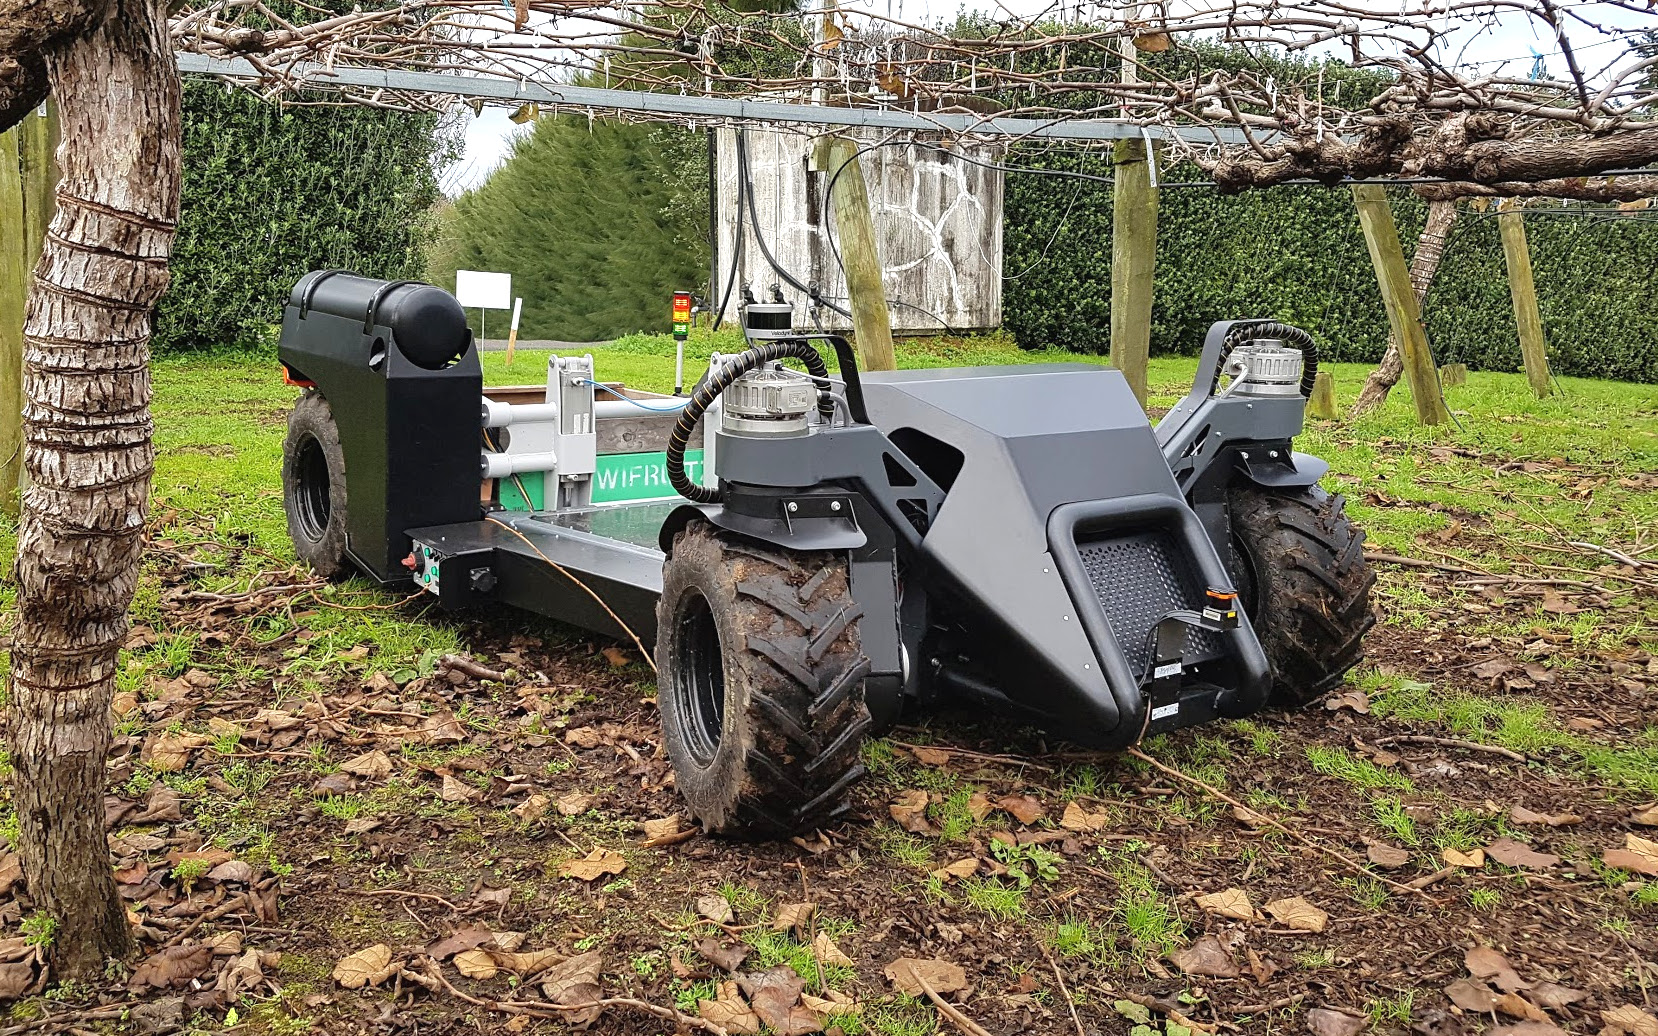
\includegraphics[width=\linewidth]{imgs/photos/suzy_general.jpg}
        \caption{
            The robot platform driving through a pergola style kiwifruit orchard.
        }
        \label{fig:suzy}
    \end{figure}

\section{Related Work}
\label{sect:review}

    \subsection{Purpose-built Autonomous Vehicles in Agriculture}

        The introduction of computers and digital camera technology during the 1980s sparked research into autonomous vehicles for agricultural use \citep{Li2009}.
        When publishing details of an autonomous vehicle in 1999, Tillett et~al.\@ cites difficulties dealing with variability in lighting and the environment as the reason no commercial ready vehicles were available at the time.
        Their vehicle combined wheel encoders, a compass, and accelerometers for odometry information.
        It also featured a camera based row guidance system.
        It was capable of spraying individual plants whilst autonomously driving at \SI{0.69}{\meter\per\second} (\SI{2.5}{\kilo\meter\per\hour}).

        Three years later, two autonomous robots designed for weed mapping and control were published \citep{Pedersen2002,Astrand2002}.
        These platforms had relatively simple chassis and drive systems as they were both at a prototype stage.
        Both featured two-wheel steering and were designed specifically for field crops.
        While both were battery powered, the platform presented by \cite{Astrand2002} could also be fitted with a combustion engine.
        The vehicle presented by \cite{Pedersen2002} was designed to follow pre-defined GPS based paths through row crops, but the authors found that this was impractical without a dedicated row guidance sensor.
        They proposed a revised design that featured a row guidance sensor, a revised drive system with four-wheel steering, and a Controller Area Network (CAN) bus for low-level communication.

        Two years later, the revised design proposed by \cite{Pedersen2002} was presented by \cite{Bak2004}.
        The authors noted that the control strategy for the four independently controlled wheels was non-trivial.
        The GPS receiver on this platform utilised Real Time Kinematic (RTK) corrections from a base station.
        RTK-GPS is capable of providing positioning with accuracies of \SI{2}{\centi\meter}.

        In 2009, details of BoniRob were published by \cite{Ruckelshausen2009}.
        Similar to the unit presented by \cite{Bak2004}, it featured a gyroscope, RTK-GPS for localisation, a CAN bus for communication, and four-wheel steering.
        What makes BoniRob particularly interesting is its ability to alter its track width by actuating the arms to which the wheels were attached.
        A \SI{2.8}{\kilo\watt} petrol generator could be mounted to the chassis, additional to its on-board batteries.
        It was capable of carrying a \SI{150}{\kilo\gram} payload in its dedicated module space.
        Like the robots before it, BoniRob was designed for use on open field crops.
        It introduced the use of both single-plane and multi-layer laser range scanning, known as lidar, for perception and row detection.
        During the previous year, some of these authors published details of a much simpler robot named `Weedy' \citep{Klose2008}, also an open field crop based sensing platform.

        Of particular relevance to this work is that of Scarfe et~al.\@ on an autonomous kiwifruit picking robot \citep{scarfe2009, Scarfe2012}.
        That work involved the creation of a hydraulically driven platform, with two-wheel steering, to which fruit harvesting arms were integrated.
        While that platform was designed to navigate kiwifruit orchards autonomously, its ability to do so was not tested.
        The platform had an internal combustion engine for on-board power generation.
        Like the platform presented here, it was designed specifically for use in kiwifruit orchards.

        Most recently, \cite{Bawden2017} present their field crop robot - Agbot~II.
        For traction it uses two driven wheels in a differential drive configuration, with two castor wheels for support.
        It is battery powered and designed to autonomously return to a shipping container sized shelter with in-built solar powered charging station.
        Their platform is comprised of two side modules and a wide centrepiece that bridges the side modules.
        These side modules contain the drive system, whereas the centrepiece is designed to be specific to the application.
        The choice of drive system has considerably reduced the robot's complexity and weight over designs previously discussed.

        \cite{Blackmore2007} envisaged significant reductions in production costs for agricultural robotics by repurposing parts already in use in the agricultural and automotive industry.
        While not a physical component, the CAN bus is one such technology borrowed from these industries.
        Most of the reviewed platforms made use of this communication system.
        Another trend is that vehicles designed specifically for open field crops favor four-wheeled over two-wheeled steering, with the exception of the Agbot II.
        However, this configuration may be less useful in an orchard environment.
        Finally, to aid development, the use of open source simulation tools allowed the creators of BoniRob to develop and test their mobility system independent from the physical hardware.


    \subsection{Sensors for Row Based Navigation in Orchards}

        Sensor combinations for orchard based row detection mostly fall into three categories; camera based, lidar based, or a combination of the two.
        The following section summarises a review of row detection efforts in orchards using these techniques.
        % Lidar come in two flavours: single-plane, and multi-layer.

        \cite{Subramanian2006} tested both camera and lidar (Sick LMS-200) based guidance systems in a citrus fruit orchard.
        Sensors were trialled separately on a tractor retrofitted with a drive-by-wire system.
        Their vehicle was able to navigate a small and simplified path using both machine vision and lidar based approaches at speeds of up to \SI{4.4}{\meter\per\second} (\SI{15}{\kilo\meter\per\hour}).
        They found that lidar proved more accurate until the lidar's data transfer rate became a limiting factor.
        The 2D camera based approach was favorable after this point.
        They suggest that combining the two systems would give more robust guidance as well as providing the ability to detect obstacles.
        No mention of the ability for the image based approach to cope with varying lighting conditions is made.

        \cite{Barawid2007} demonstrate the use of data from a single-plane lidar (Sick LMS-219) to guide a drive-by-wire tractor through an orchard.
        Their results show real-time processing of lidar data is sufficient to navigate an orchard at \SI{0.36}{\meter\per\second} (\SI{1.3}{\kilo\meter\per\hour}).

        
        In 2011, Two groups publish work on the generation of centre lines from camera data taken in orchard rows.
        \cite{He2011} uses traditional machine vision, where \cite{Torres2011} makes use of neural network based image processing.
        Both methods generate valid paths, although He et~al.\@ note that theirs may not be suitable when the environment background becomes complex.
        The neural network based approach of \cite{Torres2011} appears to cope with variations in lighting and orchard row variations.
        Also in 2011, \cite{Hansen2011} show the use of a single-plane lidar (Sick LMS-200) for vehicle localisation in an orchard.

        The work of \cite{Scarfe2012}, combined traditional camera based image processing techniques with a single-plane lidar (Sick LMS-111).
        The image based approach failed to cope with variability in lighting conditions, however the lidar proved useful for detecting the trunks and posts in kiwifruit orchards.

        \cite{Freitas2012} focused on the detection of people and bins in the rows of an apple orchard using lidar (Sick LMS-291), a low-cost inertial measurement unit, and wheel encoders.
        Their algorithm was capable of detecting each obstacle class off-line using data captured from a test orchard.

        \cite{Zhang2014} used a lidar (Hokuyo UTM-30LX) to generate maps of an apple orchard with the aid of artificial landmarks.
        They used an actuated single-plane lidar to generate multi-plane data for use in row and landmark sensing.
        Placing artificial land-marks in orchards was intended to reduce the effort required to create orchard maps for guidance systems.

        The following year, many of the same authors from  the paper presented by \cite{Zhang2014} write about their autonomous vehicle \citep{Bergerman2015}.
        It describes an electric utility vehicle converted to drive-by-wire with the addition wheel encoders for odometry and a single-plane lidar (Sick LMS-111).
        While not able to detect obstacles in real-time, their previous work processing off-line data \citep{Freitas2012} has potential to be integrated with the addition of extra on-platform computing capability.

        Most recently, \cite{Sharifi2015} write about a method to generate centre-lines from 2D images of orchard rows.
        Like the work of \cite{He2011}, the technique offers a way to generate paths from a single camera image without resorting to neural networks.
        However, their future work focuses on increasing robustness to variations in lighting conditions, which indicates issues in this area.
        They state their system has use in being complementary to lidar based navigation.

        The experiences of \cite{Scarfe2012}, and others, indicate that a lidar outputs data that requires less post-processing to be robust.
        The use of lidar has seen two of the reported vehicles navigate autonomously through orchard environments, which is encouraging.
        Other reports suggest that traditional image based processing for navigation fails when the scene becomes complex or significant variations in lighting occur.
        Combining cameras with neural network based processing increases the robustness to environmental complexities, such as light or clutter, at the expense of increased computation.
        % Common among these vehicles is the use of sensor fusion, whereby data from multiple sensors is merged and filtered.
        % This provides a way to combine the advantages of multiple sensor types, and the benefit of redundancy  into a single computation space.

        With regards to the use of RTK-GPS in guidance systems, Slaughter et~al.\@ points out the trade-off of requiring an ``unobstructed `view' of the sky from all parts of the field'' \citep{Slaughter2008}.
        % Additionally, multi-path signal propagation caused by nearby foliage or the geometry of the land itself presents its own mode of failure \citep{Durrant-Whyte2005}.
        A feasibility analysis by \cite{Pedersen2006} highlighted the use of RTK-GPS systems as a significant cost in yearly subscriptions alone.
        \cite{Durrant-Whyte2005} describe one failure mode of GPS being multi-path signal propagation caused by nearby foliage or the geometry of the land itself.
        % This requirement can not be satisfied under the canopy of a kiwifruit orchard which are usually surrounded by tall wind-breaking hedges.
        % \cite{Torii2000} suggests a combination of both RTK-GPS and machine vision systems to be the most promising system going forward based on reductions in costs and increases in performance of these systems.
        While \cite{Li2009} concludes that either GPS and machine vision, or GPS and lidar will be used together as a development trend.
        Based on the high ongoing cost and increased reception requirements, we discount the use of an RTK-GPS system, but still consider the use of GPS in-orchard.

\section{Platform Design}

    \subsection{Vehicle Configuration}
    \label{sect:mechanical}

        \begin{figure}[htb]
            \centering
            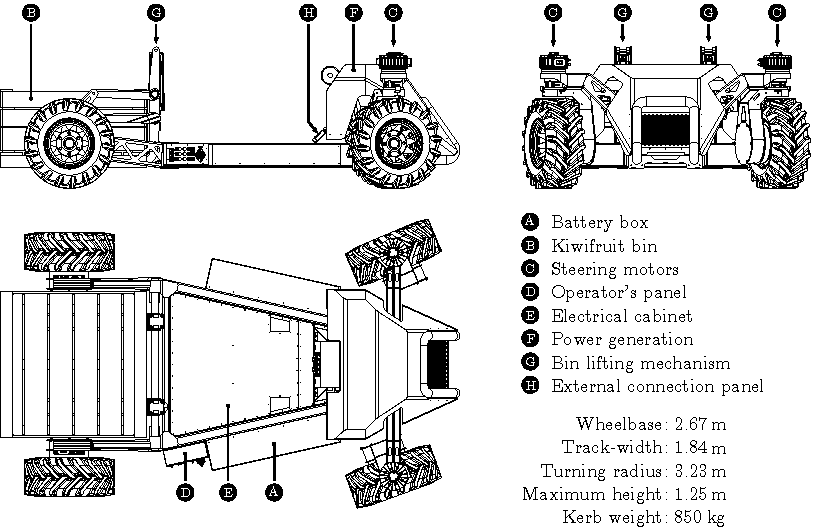
\includegraphics[width=\linewidth]{imgs/profile_views/AMMP-All-Labelled.pdf}
            \caption{Profile drawings of the robotic platform with kiwifruit bin.}
            \label{fig:AMMP}
        \end{figure}

        Modules designed to be carried by our platform require clearance from the canopy in addition to the height they occupy themselves.
        A kiwifruit canopy typically varies in height from \SI{1.3}{\meter} to \SI{1.7}{\meter} between orchards.
        To maximise the space available to these modules the platform must be low-slung at the point they attach.
        Figure \ref{fig:AMMP} illustrates the platform's design, with module area allocated between markers `G' and `H' in the side view (top left).
        The top surface of the chassis in this region is \SI{360}{\milli\meter} above the ground.

        The platform's steering geometry is Ackermann based.
        Steering angles are controlled using the front two wheels which are actuated independently by brushless AC motors.
        The ability to actuate the angles individually simplifies the mechanical geometry needed to coordinate steering, particularly at extreme angles.
        Both steered wheels have the freedom to rotate \SI{330}{\degree}, artificially limited by mechanical stops.
        This allows the vehicle to pivot about the centre of the rear wheels during tight turns, where its turning circle would be twice the vehicle's length.
        % This range in steering angle allows the vehicle to place the centre of rotation at the mid-point between its rear wheels during its tightest turn.
        % At this steering angle, .
        Implementing four wheel steering would allow the centre of rotation to move to the centre of the vehicle, halving the turning circle.
        However, headlands in kiwifruit orchards are sized for tractors to turn between rows; tractors with two-wheel steering geometries.
        Implementing a two wheeled steering system removes the need to develop the ``non-trivial'' control strategies and increases the usable platform area.
        A differential drive, or skid steer, system was expected to cause ground damage to a level considered unacceptable to orchard owners.

        Bin lifting forks are fitted to the area between the rear wheels.
        This area is sized to accommodate a kiwifruit bin.
        The lifter is actuated by two vertically mounted pneumatic cylinders and is controlled by a standard pneumatic valve block.
        In future, the platform is expected to have the ability to pick and place bins autonomously while operating in an orchard.

        Other than its tires, the platform has no suspension.
        It features a front pivoting axle that ensures a minimum of three wheels are always in contact with the ground.
        Each wheel is mounted directly to a 40:1 fixed-ratio planetary gearbox connected to a permanent magnet brushless AC motor.
        This specific gearbox-motor combination limits the platform to a maximum speed of \SI{10}{\kilo\meter\per\hour}.
        The lack of suspension is not an issue when operating in orchards at this speed.
        In total, the drive system can continuously deliver \SI{25.6}{\kilo\watt} of power and \SI{3.3}{\kilo\newton\meter} of torque.
        Based on these specifications it is capable of accelerating from a stand-still to its maximum speed at an incline of \SI{20}{\degree} whilst carrying a \SI{600}{\kilo\gram} payload in \SI{2.0}{\second}.

        A power generation unit comprised of a petrol engine (Honda GX-690), air compressor (Rotorcomp NK-1), and electrical generator (Heinzmann PMSG-150) sits over the front pivoting axle.
        The drive shafts of the three units are connected with a heavy-duty timing belt.
        The engine, compressor, and alternator can be controlled electronically from an embedded controller module.
        This power generation controller module is connected to the rest of the system via CAN bus.
        
        Fuel and compressed air tanks sit over the right-hand rear wheel, visible in figure \ref{fig:suzy}.
        Electrical energy from the power generation unit is fed directly into the battery modules in a series-hybrid configuration. 
        The fuel tank can hold approximately \SI{60}{\litre} of petrol, allowing the platform to operate continuiously for an estimated period of up to \SI{48}{\hour} under light loads.
        Two battery modules attached to the sides of the chassis each house fifteen lithium-iron-phosphate (LiFePO$_{\text{4}}$) batteries connected in series.
        The batteries (Winston/Thundersky WB-LYP90AHA) have a nominal voltage of \SI{3.2}{\volt} and a capacity of \SI{90}{\ampere\hour}.
        Together they provide a nominal bus voltage of \SI{96}{\volt} and a total electrical capacity of \SI{8.64}{\kilo\watt\hour}.
        From this, on-board power supplies can continuously deliver \SI{2.8}{\kilo\watt} at \SI{12}{\volt}DC, \SI{3.8}{\kilo\watt} at \SI{24}{\volt}DC, and \SI{3.5}{\kilo\watt} at \SI{240}{\volt}AC, simultaniously, while driving.
        A connection panel near the front of the platform holds the weather-sealed plugs through which these outputs are accessible.

        Unloaded, the machine has an estimated mass of \SI{850}{\kilo\gram}, including the power generation unit and batteries.
        It is capable of carrying a \SI{1000}{\kilo\gram} payload.
        The mass of a standard bin of kiwifruit can be as much as \SI{400}{\kilo\gram}, leaving \SI{600}{\kilo\gram} for modules.
        % With that load, the platform's maneuverability and ability to brake or accelerate was not noticeably affected.

    \subsection{System Architecture}
    \label{sect:architecture}

        \begin{figure}[htb]
            \centering
            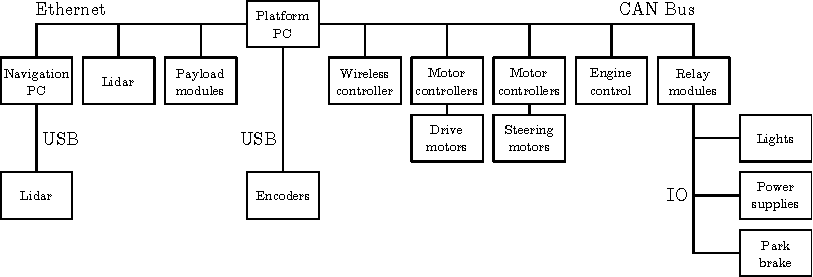
\includegraphics[width=\linewidth]{imgs/system_diagram/diagram_v3.pdf}
            \caption{Hardware level system diagram showing the types of interfaces and relative relations on the platform.}
            \label{fig:system_diagram}
        \end{figure}

        This section briefly explains the hardware and software architecture of the platform.
        Standardised protocols and software frameworks are employed where possible, supplemented with custom solutions where needed.

        The platform is centrally controlled by an x86 based small-form-factor PC running Ubuntu 16.04 server.
        That computer is connected to an on-board Ethernet network and CAN bus.
        Low-level sub-systems on the platform such as motor controllers and relays are connected to this `Platform PC' via CAN bus.
        Figure \ref{fig:system_diagram} shows a simplified arrangement of connections between each module.
        
        A second computer dedicated to the processing of sensing data for autonomous navigation is connected to the platform PC via Ethernet.
        It too is an x86 based PC running Ubuntu, but uses a microATX form-factor motherboard with a Nvidia GTX 1070 graphics card.
        This PC is responsible for computing all aspects of autonomous navigation, such as connecting to sensors, filtering and processing data, generating drive commands, and communicating with the platform PC.
        The graphics card is used to accelerate neural network algorithms and some image processing functions.

        The open source Robotic Operating System (ROS) is used to facilitate communication between both computers and between software nodes within each machine.
        Figure \ref{fig:system_diagram_software} shows a simplified passage of information entering through navigation sensors, being passed between various nodes, and finally being fed to the motor controllers.
        % For simplicity it omits interface nodes, those used solely to interface the device to the ROS network.
        To maximise code reusablility, each device on the platform has its own ROS node dedicated to publishing device data or subscribing to generated device commands.
        Examples of such devices being interface adapters, motor controllers, wireless controllers, lidar, and encoders.
        Nodes are also used to transform or perform calculations on data and pass it between nodes written in either C++ or Python.
        For instance, as figure \ref{fig:system_diagram_software} shows, the `Ackermann kinematics' node transforms steering input data to individual wheel velocities and positions based on Ackermann calculations.
        This node could easily be swapped out for a different translator node during run-time without disturbing the system.

        Relay modules allow the platform PC to toggle power to on-board power supplies, motor controllers, park-brakes, and lights.
        These modules also monitor the timing of synchronisation messages transmitted by the platform PC onto the CAN bus, which should occur every \SI{20}{\milli\second}.
        Once a module detects an absence of synchronisation messages for \SI{100}{\milli\second} or longer it enters a defined error state.
        % If the module does not receive a syncronisation message for \SI{100}{\milli\second} it will enter an error state.
        That state will result in the motor controllers and on-board power supplies being shut-off and the park brakes engaged.
        Since power is required to disengage the park brakes, this equates to `shutting-off' the brake release mechanism.
        CAN bus monitoring ensures that the system is automatically shut down in a timely manner should the platform PC become unresponsive.

        \begin{figure}[htb]
            \centering
            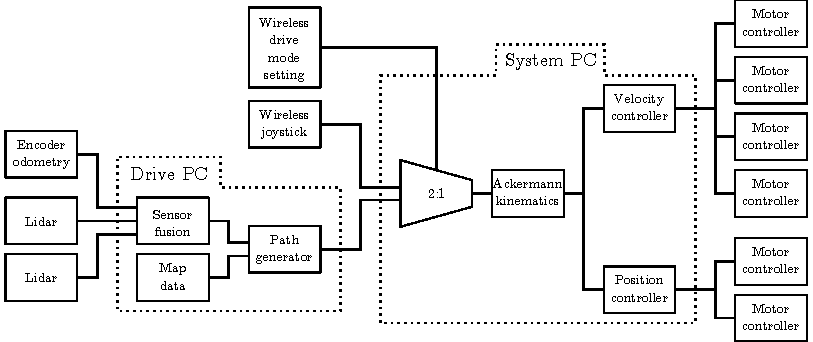
\includegraphics[width=\linewidth]{imgs/system_diagram/software.pdf}
            \caption{Simplified system diagram (partial) showing node connectivity used for manual and autonomous platform control.}
            \label{fig:system_diagram_software}
        \end{figure}

        In addition to the drive commands generated by the navigation system, a safety rated wireless controller (HBC Radiomatic Eco) lets the operator input drive commands via joystick.
        The joystick also has a mode switch that allows the operator to select between manual and autonomous control, and an emergency stop button.


\section{Navigation Sensors}
\label{sect:sensors}
    The choice of sensors incorporated into a platform determines which approaches are available for navigation and object detection.
    This section details the sensor selection and navigation algorithms specific for use in kiwifruit orchards.
    We begin by selecting a number of sensors considered appropriate for navigation in this environment.
    Following this, we test each sensor's ability to capture relevant data.
    Finally, we test the performance of promising sensors with prototype navigation and object detection algorithms.
    An evaluation of each sensor is discussed in the context of orchard based navigation.

\subsection{Sensor Selection}

    As the drive motors have in-built wheel encoders, basic odometry data is already available.
    Encoders on driven wheels can give false readings if wheel slip occurs so should not be used for odomentry alone.
    However, the data they provide can be used to assist with mapping, localisation, and provide velocity feedback.

    Other sensors considered for inclusion are outlined in table \ref{table:sensor_comparison} with their associated issues.
    Factors considered were strengths and weaknesses in the context of orchard use, reported usage in literature, and availability at a suitable price.
    The investigation highlighted both lidar and 2D cameras as offering high functionality for navigation and object detection.
    Time-of-flight cameras were a compelling option based on a cost-benefit analysis; especially if cheaper units work in sunlight.
    Because localisation is such a key functionality, the performance of GPS has also been evaluated.
    % The following sections detail our experiences while trialling these sensors.

    \begin{table}[htbp]
        \centering
        \footnotesize
        \begin{tabular}{ l l}
            \textbf{Sensor Type}      &\textbf{Possible Issues} \\ \hline
            GPS receiver              & Prone to signal loss from surrounding foliage\\  \hline
            Inertial Measurement Unit & Error accumulation and thermal drift\\ \hline
            Digital Compass           & Can be disturbed by nearby structures\\ \hline
            Encoder                   & Error accumulation \\ \hline
            Lidar                     & Reduced visibility in fog and heavy rain \\ \hline
            Time of Flight Camera     & Reduced visibility in sunlight, fog and heavy rain \\ \hline
            Camera                    & Reduced visibility in fog or direct sunlight \\ \hline
            Thermal Camera            & Reduced visibility in conditions of low thermal contrast\\ \hline
        \end{tabular}
        \label{table:sensor_comparison}
        \caption{Sensor types considered for inclusion on the platform.}
    \end{table}

% \subsection{Data Collection and Inspection}
 %    The sensors that seemed important to test, based on both the literature survey and the cost-benefit analysis were lidar, cameras and GPS.
	% In addition, time of flight cameras were considered, because they seemed to be a compelling option based on the cost-benefit analysis; especially if some of the less expensive models were found to work well in sunlight.
	% It was also decided that encoders would be tested in favour of using an IMU because the encoders were built into the AMMP motors.
	% Some data was collected from each sensor in order to decide which sensors to prototype algorithms for.

    \subsubsection{In-orchard GPS Evaluation}
        Two GPS modules were evaluated: a Ublox Neo-M8N module and an OmniSTAR 5120VBS with AX0 series antenna.
    	Both were connected to a Beaglebone Black single board computer via serial connection for data acquisition.
        The Ublox module was selected for its high sensitivity, internal low noise amplifier, and active circuitry for its ceramic patch antenna.
        The OmniSTAR receiver was chosen for its external high-gain antenna (34 dB) which claims multi-path rejection.

        The testing procedure first involved planning a path through a single row of a kiwifruit orchard and plotting it on a satellite map.
        Waypoints were placed along the row at the location of posts used to hold the canopy's structure.
        Relative distances between these waypoints were measured with a tape measure and recorded.
        The receivers were then tested separately over the course of approximately two hours.
        Before testing, each unit was powered up and given \SI{30}{\minute} to initialise in an open area near the kiwifruit orchard.
        During testing, each unit was walked slowly along the pre-determined path with stops at each waypoint to provide time for a positional fix.
        The path was approximately \SI{500}{\meter} in length and took approximately \SI{15}{\minute} to complete, including stops at each waypoint.
        Waypoints were spaced at intervals of \SI{5.5}{\meter} along the row.

        \begin{figure}[htb]
            \centering
            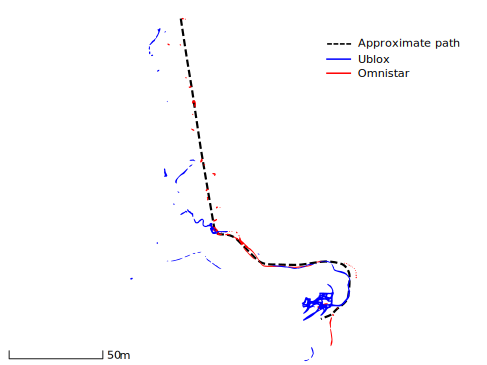
\includegraphics{imgs/gps_path/gps_path.pdf}
            \caption{
                Aerial view of the path taken through the test orchard and the captured GPS data.
            }
            \label{fig:gpsResults}
        \end{figure}

        The path followed, and the corresponding GPS locations collected from the receivers, is presented in figure \ref{fig:gpsResults}.
        It should be noted that data has been recorded for the round-trip so represents two passes along the path.
        It was noticed during testing that the signal quality lights on both GPS receivers regularly indicated a loss of signal.

        The Omnistar receiver appears to track the approximate path well, but the data is sparse with regular loss of signal after entering the orchard.
    	The Ublox receiver collected more data, but was much less accurate.
        It may be possible to use a unit such as the Omnistar, which provided fewer but more accurate readings, as a sanity check for an approximate location within orchards.
        Overall the units could not be relied on for localisation in this environment.
        Based on these results, we consider GPS receivers similar in performance to those trialled to be unsuitable for use in kiwifruit orchards.

    \subsubsection{In-orchard Lidar Evaluation}
        Three lidar were evaluated, two single-plane and one multi-layer.
        The two single-plane lidar were the Hokuyo UTM-30LX and a SICK LMS111.
        The multi-layer lidar is a Velodyne VLP-16 which has 16 horizontal \SI{360}{\degree} planes spread over \SI{15}{\degree} vertically.
        Data was collected from each lidar by driving through orchard rows with the sensor placed midway between the ground and canopy (approximately \SI{0.8}{\meter} off the ground).

        \begin{figure}[htb]
            \centering
            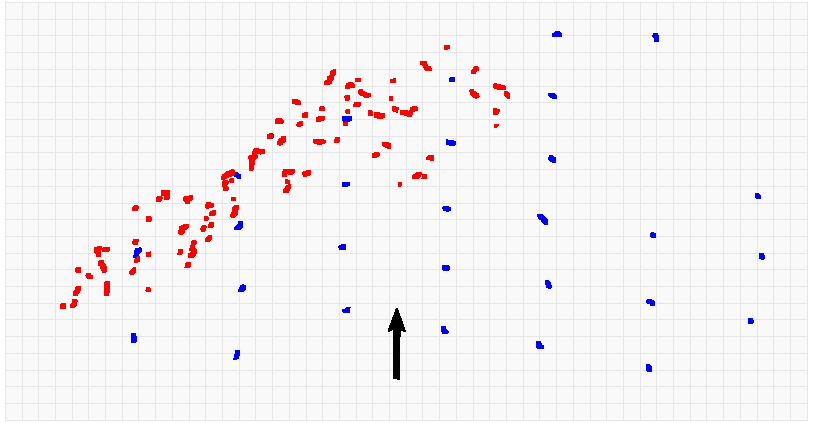
\includegraphics[width=\linewidth]{imgs/canopy_data/canopy_data.pdf}
            \caption{
                Captured lidar data showing the non-structural points reflected by the canopy (indicated by red markers) and structural points from tree trunks and posts (blue markers).
                The arrow indicates the position and heading of the platform at the time of capture.
            }
            \label{fig:canopyDataCloud}
        \end{figure}

        The intention was to use lidar as a means of detecting structure defining features of the orchard, such as posts, trunks and hedges.
        Detecting these features should allow for row boundary detection, or general mapping and localisation.
        However, both single-plane lidar produced clouds of unstructured data amongst the structured features, as shown in figure \ref{fig:canopyDataCloud}.
        This was caused by the lidar's scan plane intercepting with the canopy whilst driving over convex terrain.
        Similarly this issue arose on concave terrain where the plane intercepted with the ground, as depicted in figure \ref{fig:concaveSlope}.

        \begin{figure}[htb]
            \centering
            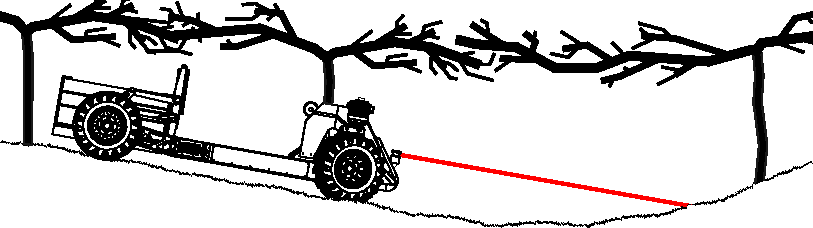
\includegraphics[width=\linewidth]{imgs/concave_slope/concave_slope_v4.pdf}
            \caption{
                On concave slopes the lidar scan plane intercepts with the ground instead of trunks or posts.
                The dashed line shows a horizontal plane coming from the the lidar.
                Dotted lines represent the upper and lower layers taken from the multi-layer lidar.
            }
            \label{fig:concaveSlope}
        \end{figure}

        This issue was reduced by the use of a multi-layer lidar and post-processing.
        Because of the 16 layers, it is possible to select the scan layer that gives the most useful viewing range.
        Referring to figure \ref{fig:concaveSlope}, that would correspond to the dotted line above the horizontal (dashed) line which intercepts with a row defining feature (tree trunk).

        It was decided that a multi-layer lidar would be best suited for navigation due to its ability to to see more distant features while driving on undulating ground.
        A single-plane lidar could still be used at short range as an independent channel of processing for redundancy or obstacle detection.
        For the platform, a single-plane lidar has been fitted to the front of the vehicle as an object detector for possible collisions, and a multi-layer lidar has been fitted for use in navigation and general object detection.


    \subsubsection{In-orchard Camera Evaluation}
        \label{sect:camera_evaluation}

        Three varieties of camera were tested: time-of-flight, 3D stereoscopic, and traditional 2D cameras.

        The time-of-flight based camera was the Basler TOF640-20GM-850NM.
        It provides range, intensity, and confidence data at a resolution of 640 by 480 pixels.
        This specific model was chosen as it had previously proved useful when collecting depth data of kiwifruit canopies.
        During that time it had been operated under different lighting conditions and exhibited minimal occurrences of data loss.
        However, these tests revealed that in both direct sunlight and overcast conditions there was significant data loss.

        The 3D stereo camera tested was an Intel RealSense R200.
        It combines a stereo pair of infra-red cameras with a colour camera.
        Additionally, it features an infra-red projector as a means of adding texture to objects in its field of view to assist with stereo processing.
        The appealing characteristics of this sensor were its low cost and its claim of being long-range and able to work outdoors.
        However, in both overcast and sunny conditions it suffered from a complete loss of range data.

        Finally, 2D-cameras were trialled.
        These were the Basler Dart daA1600-60uc, Flir CM3-U3-13S2C-CS, and Logitech C920 cameras.
        Like the lidar tests, each camera was driven through the orchard at a height of \SI{0.8}{\meter} from the ground.
        The Logitech C920 suffered from significant motion blur.
        Being a consumer grade web-camera this was not surprising; it also lacks a hardware trigger interface.
        A hardware trigger becomes important if the camera is used in stereo vision applications.
        The Basler and Flir cameras both produced images of sufficient quality.
        The Basler offering was favored for its later model image sensor.

        Overall, the more industrial 2D camera images were deemed suitable for object detection and classification.
        This was verified by processing the data using readily accessible detection algorithms such as convolutional neural networks discussed next.
        Both the time-of-flight and 3D stereoscopic camera systems were deemed unsuitable based on the occurrences of data loss while operating in sunlight or overcast conditions.

\subsection{Sensor Demonstration by Prototype Algorithm}

    Basic tests indicated that multi-layer lidar and 2D cameras were best suited for use as primary in-orchard navigation sensors.
    Further testing with prototype navigation algorithms ensured that these apparent sensor benefits translated into practical advantages.

    The three goals for the navigation system are:
    \begin{itemize}
        \item object detection and classification,
        \item mapping and localisation, and
        \item orchard row tracking.
    \end{itemize}
    To validate that the sensors could perform these functions, three prototype navigation algorithms have been created.

    \subsubsection{Object Detection and Classification}

        % Object detection and classification was firstly prototyped fully on the camera data.
        Based on existing success using Convolutional Neural Networks (CNN) for image processing tasks \citep{LeCun2015}, a camera based system was chosen for object detection and classification.
    	The network architecture chosen was FCN-8s \citep{long2015}.
        It is a neural network made of convolutional layers without fully connected layers.
        % convolutional layers at the input and fully connected layers at the output.
    	FCN-8s performs semantic segmentation, which is per pixel classification of images.

        To train the FCN-8s network, the same image dataset used to assess camera performance earlier was hand labeled.
    	Labeling involved drawing object outlines in each image, filling those outlines with colours corresponding to the object's type, and filling any non-labeled areas with black.
        Each image was then converted to an indexed colour file format.
    	An example of an original image and its corresponding label image is shown as figure \ref{fig:segImgLabelPair}.

        \begin{figure}[htb]
            \centering
            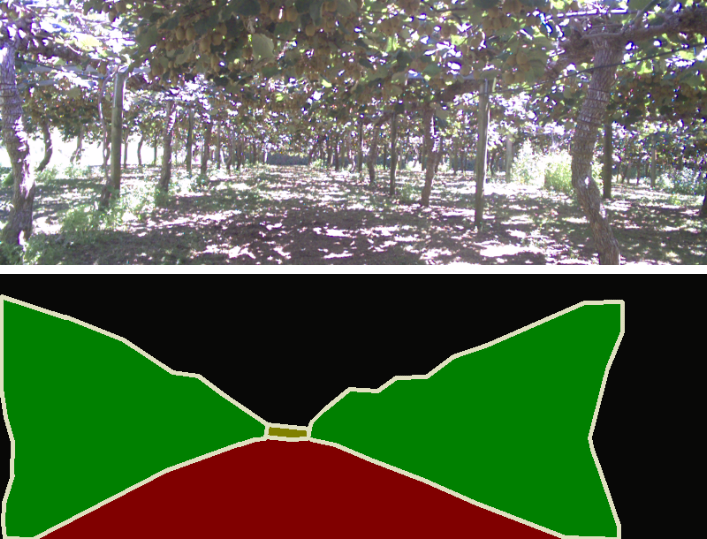
\includegraphics[width=\linewidth]{imgs/photos/segImgLabelPair_trimmed.png}
            % \includegraphics[width=\linewidth]{imgs/photos/segImg_sideBySide.png}
            \caption{
                An input image (top) and labelled output (bottom) used to train the semantic segmentation network.
            }
            \label{fig:segImgLabelPair}
        \end{figure}

        \begin{figure}[htb]
            \centering
            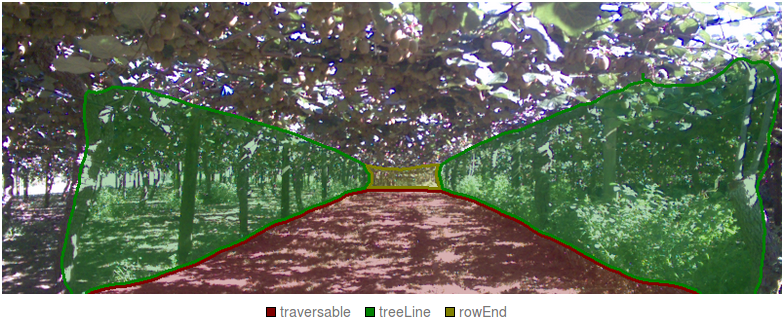
\includegraphics[width=\linewidth]{imgs/photos/semSegRowResults.png}
            \caption{
                An example inference result from the trained FCN-8 network.
            }
            \label{fig:semSegRowResults}
        \end{figure}

        Initially, individual trees and posts in the kiwifruit orchard were labeled.
    	It was later found that labeling the entire tree-line as a single class gave more robust results.
    	Objects labeled for this algorithm are:
        \begin{enumerate}
        \item traversable space (labeled as red),
        \item treelines (labeled as green), and
        \item the end of the current row (labeled as tan).
        \end{enumerate}
        Traversable space was defined as the ground area that the platform could drive directly to without collision.
        These labelled images were then used to train the FCN-8s network.
    	Sample output from the trained network is presented as figure \ref{fig:semSegRowResults}.

    \subsubsection{Mapping and Localisation}
        An existing Simultaneous Localisation And Mapping (SLAM) package was used to test the multi-layer lidar.
        The package used was Gmapping \citep{Grisetti2007}, implemented as a ROS package \citep{Gerkey2010}.
    	Required input for Gmapping is odometry data and a single plane of lidar data.
        The obometry data was provided by the platform's in-built wheel encoders.
    	
        \begin{figure}[htb]
            \centering
            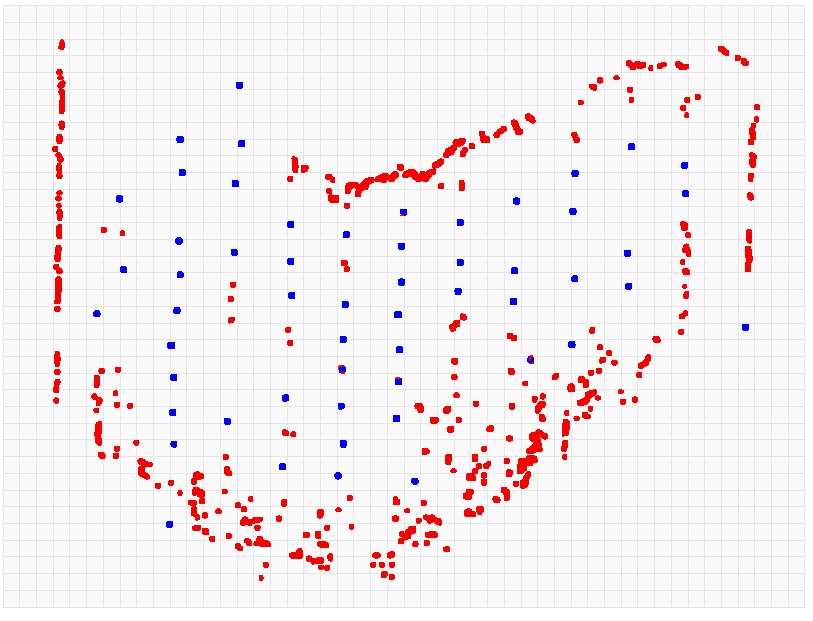
\includegraphics[width=\linewidth]{imgs/single_plane_extraction/single_plane_extraction.pdf}
            \caption{
                Processing of multi-layer lidar data into a single plane equivalent.
                Blue points are those selected by the algorithm for further processing, whereas red points are rejected.
            }
            \label{fig:singlePlaneExtraction}
        \end{figure}

        As the lidar (Velodyne VLP-16) has 16 scanning layers, a conversion was necessary to produce the single plane of data required by Gmapping.
        The simplest conversion from multi-layer data to a single plane would be to select one of the available planes and discard the remaining data.
        However, that approach would loose any benefit offered by the multiple scanning layers.
        Instead, filtering the multi-layer data into a single plane was done by examining data from the centre four scan layers at each azimuth.
        With this algorithm, if the range difference between all four points at a single angle falls below a certain threshold, the closest point is returned.
        Alternatively, if the spread in points is above the threshold, no points are returned.
        This eliminates points from sloped or varying surfaces while still returning points from objects with vertical structure.
        The effect of this is that the orchard's structural elements remain visible, but ground and canopy information are removed.

        \begin{figure}[htb]
            \centering
            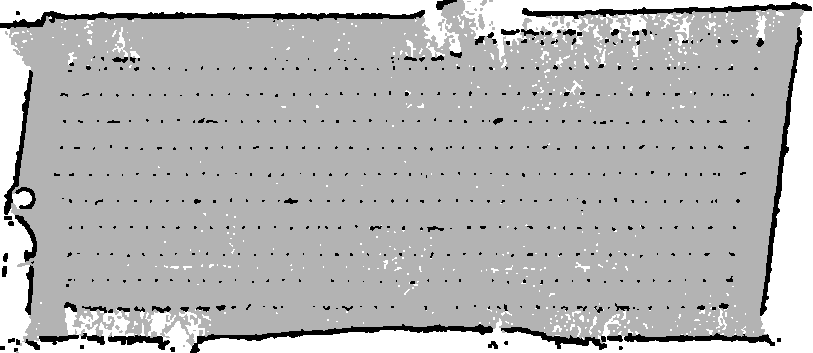
\includegraphics{imgs/gmapmap/gmapmap.pdf}
            \caption{
                A resulting SLAM based map of a kiwifruit orchard created using Gmapping.
                Data for the map was collected by traversing four of the orchard's ten rows.
                Odometry information has been taken from wheel encoders and a multi-layer lidar (Velodyle VLP-16).
            }
            \label{fig:gmapmap}
        \end{figure}

        The filtered points are then fed into Gmapping as a single plane with data from the platform's wheel encoders.
        Figure~\ref{fig:singlePlaneExtraction} shows the mothod's ability to filter structural elements from data containing significant canopy and ground reflections.
        Using this method, a SLAM based map of the orchard was created and is presented as figure \ref{fig:gmapmap}.


    \subsubsection{Kiwifruit Orchard Row Tracking}
        \label{sect:row_tracking}

        Our final navigation test requires interpreting the orchard's structure for the purpose of path generation.
        For this, a row guidance system was developed and tested.
        It uses the multi-layer to single-plane data filtering technique discussed previously.
        This algorithm also makes use of the on-board wheel encoders.
        Details of this algorithm have been published separately \citep{Bell2016}.
        The key function of this algorithm is computing the angular offset of the platform from the row's centre-line.

        A visualisation of data captured whilst navigating the kiwifruit orchard is presented as figure \ref{fig:lastLidarFrame}.
        The method does not perform SLAM, so the visualised data represents only the current sensor input, i.e., previous sensor data is not considered.
        Figure \ref{fig:lastLidarFrame} shows that while the algorithm is not perfect, it does perform reasonably well at identifying orchard structure and generating valid headings.

        \begin{figure}[htb]
            \centering
            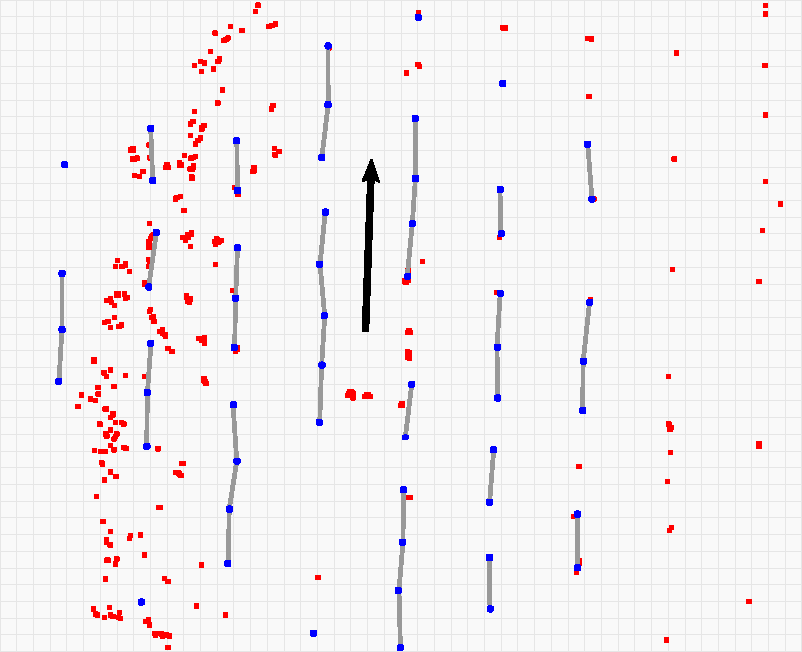
\includegraphics[width=\linewidth]{imgs/row_following/row_following_narrow.pdf}
            \caption{
                Row detection from multi-plane lidar data.
                Red points indicate non-structured data that have been ignored.
                Blue points indicate orchard structure data used for row navigation.
                Grey lines link orchard structure points by their nearest neighbours.
                The black arrow represents the centreline of the row current row.
            }
            \label{fig:lastLidarFrame}
        \end{figure}

\subsection{Sensor Selection Conclusions}
    The results from prototyped algorithms indicate that the multi-layer lidar combined with encoder feedback are useful for performing mapping and localisation.
    This combination alone has proven successful for autonomous driving in kiwifruit orchards.
    A combination of 2D cameras and neural networking was suitable for object detection and classification.
    Further research toward using this as a means of generating a path for row following is underway and is expected to be published in future.

	% Object detection using a combination of colour cameras and neural networks in kiwifruit orchards .
	% Based on these results it was decided to continue testing cameras and multi-plane lidar as the primary sensors for the navigation system.
    % The autonomous driving algorithm described has been used to drive 20 km autonomously on three different robot platforms, including the AMMP, in two different kiwifruit orchards.
    % This driving was performed using just lidar and encoder data.


\section{Autonomous Driving}
\label{sect:autonomous}
    Using the row following algorithm developed for sensor testing, map based autonomous navigation of a kiwifruit orchard was implemented.
    Two key additions were required for the platform to navigate the orchard unassisted: the detection of a row's end and a method for turning between rows.

    The detection of a row's end is made by detecting a minimum volume of free space above the multi-layer lidar (Velodyne VLP-16).
    Put simply, this equates to searching for a lack of canopy above the robot.
    This approach makes use of the multi-layer lidar, where layers above the horizontal are used as an `absence of canopy' detector.

    Turns between rows are performed by driving a series of set curvature movements while simultaniously performing lidar based obstacle avoidance.
    The series of set turns are recorded in a map file which are followed by the platform at the end of each row.
    A turn sequence sees the platform drive with a given steering angle for a given distance or until a given heading is achieved.
    Each row turn can contain any number of these sub-manovours.
    On completion of a turn, row following behavior is resumed which guides the platform through the row to the next turn.
    Figure \ref{fig:suzy_turning} shows the platform performing a row-end turn while under autonomous control.

    \begin{figure}[htb]
        \centering
        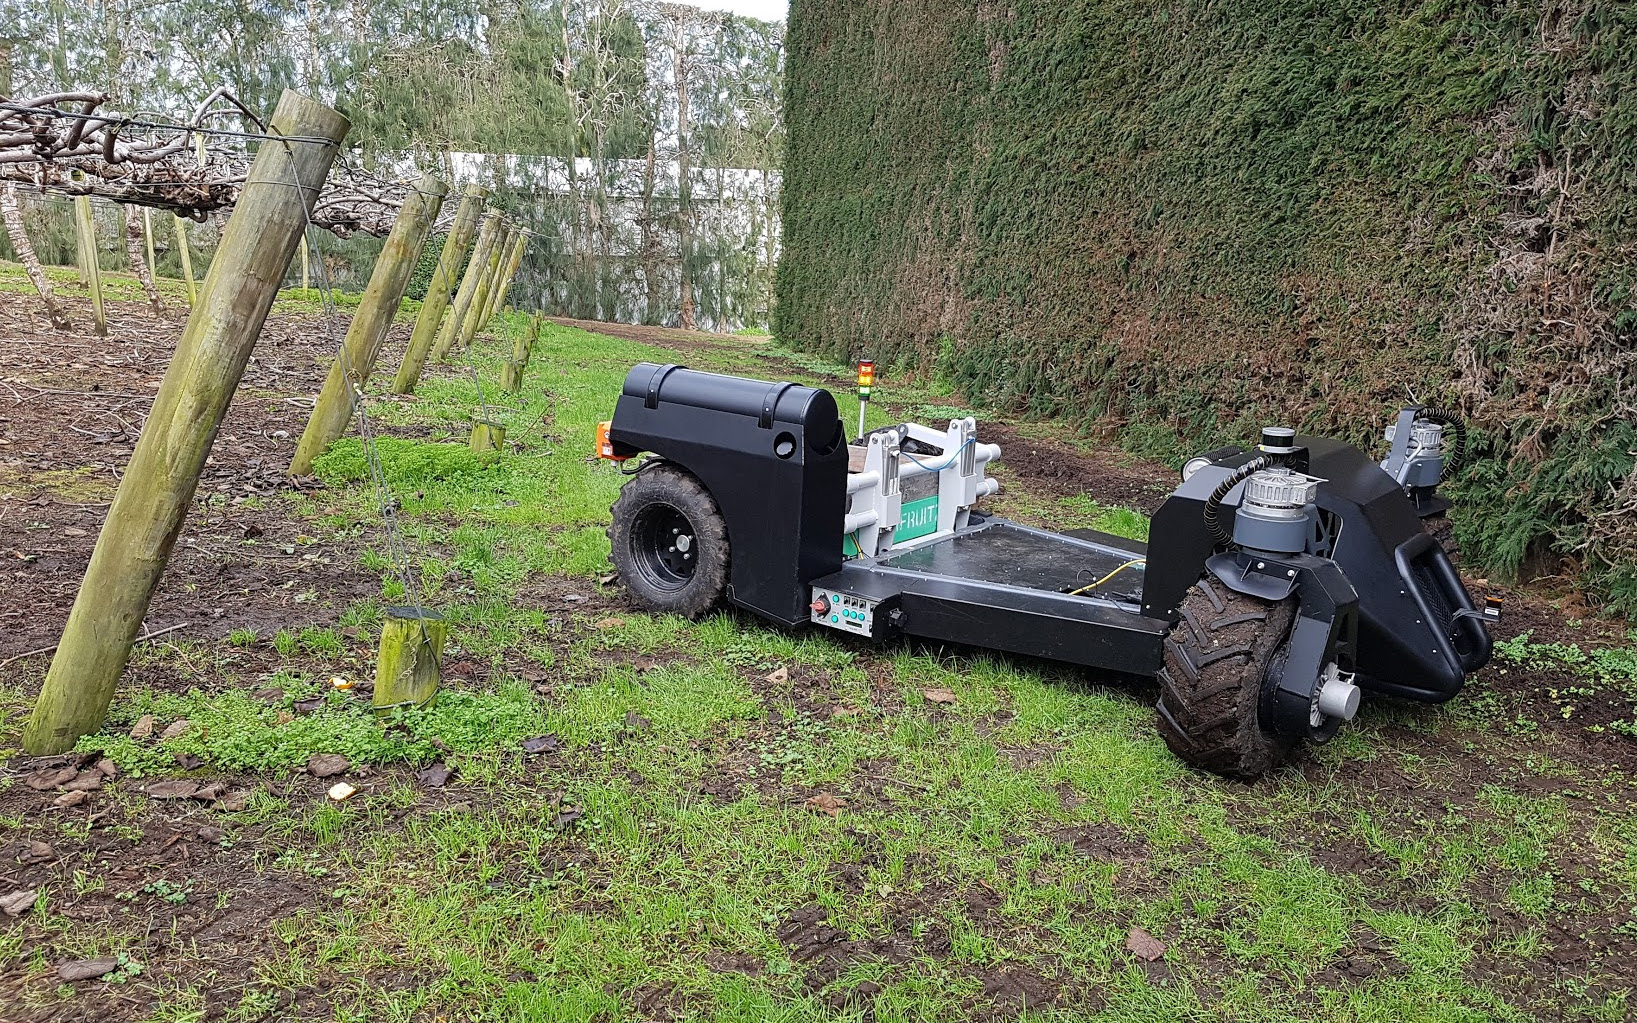
\includegraphics[width=\linewidth]{imgs/photos/suzy_turning.jpg}
        \caption{
            Photo of the platform performing a row-end turn in the headland area of a kiwifruit orchard while under autonomous control.
        }
        \label{fig:suzy_turning}
    \end{figure}

    Using the approaches developed here the platform is routinely able to navigate the test orchard block unassisted.
    This block is over \SI{1}{\kilo\meter} in total traversable length, spread over 10 rows.
    The developed algorithm has been used to autonomously control this platform and two smaller platforms through \SI{20}{\kilo\meter} of kiwifruit orchards.


\section{Conclusion}
    In this work, a platform designed specifically for driving through pergola style kiwifruit orchards has been presented.
    The platform has the capability of carrying a payload of up to \SI{1000}{\kilo\gram} through these orchards with minimal performance degradation.
    Sensors suitable for autonomous navigation have been selected, trialled and demonstrated as being useful as a means of navigating in this environment.
    Convolutional neural networks applied to monocular images proved to be a promising technique for row navigation and further work in this area is under-way.
    By processing multi-layer lidar data the platform presented here can reliably navigate an orchard block without human intervention.


\section*{Acknowledgements}
This research was supported by the New Zealand Ministry for Business, Innovation and Employment (MBIE) on contract UOAX1414.
The authors acknowledge contributions from Phillip Ross, Gordon Neshausen, Josh Barnett, and Erin Simms who were involved with the design and fabrication of the platform, and assistance testing and training neural networks from Nicky Penhall.

%% The Appendices part is started with the command \appendix;
%% appendix sections are then done as normal sections
%% \appendix

%% \section{}
%% \label{}

%% References
%%
%% Following citation commands can be used in the body text:
%%
%%  \citet{key}  ==>>  Jones et al. (1990)
%%  \citep{key}  ==>>  (Jones et al., 1990)
%%
%% Multiple citations as normal:
%% \citep{key1,key2}         ==>> (Jones et al., 1990; Smith, 1989)
%%                            or  (Jones et al., 1990, 1991)
%%                            or  (Jones et al., 1990a,b)
%% \cite{key} is the equivalent of \citet{key} in author-year mode
%%
%% Full author lists may be forced with \citet* or \citep*, e.g.
%%   \citep*{key}            ==>> (Jones, Baker, and Williams, 1990)
%%
%% Optional notes as:
%%   \citep[chap. 2]{key}    ==>> (Jones et al., 1990, chap. 2)
%%   \citep[e.g.,][]{key}    ==>> (e.g., Jones et al., 1990)
%%   \citep[see][pg. 34]{key}==>> (see Jones et al., 1990, pg. 34)
%%  (Note: in standard LaTeX, only one note is allowed, after the ref.
%%   Here, one note is like the standard, two make pre- and post-notes.)
%%
%%   \citealt{key}          ==>> Jones et al. 1990
%%   \citealt*{key}         ==>> Jones, Baker, and Williams 1990
%%   \citealp{key}          ==>> Jones et al., 1990
%%   \citealp*{key}         ==>> Jones, Baker, and Williams, 1990
%%
%% Additional citation possibilities
%%   \citeauthor{key}       ==>> Jones et al.
%%   \citeauthor*{key}      ==>> Jones, Baker, and Williams
%%   \citeyear{key}         ==>> 1990
%%   \citeyearpar{key}      ==>> (1990)
%%   \citetext{priv. comm.} ==>> (priv. comm.)
%%   \citenum{key}          ==>> 11 [non-superscripted]
%% Note: full author lists depends on whether the bib style supports them;
%%       if not, the abbreviated list is printed even when full requested.
%%
%% For names like della Robbia at the start of a sentence, use
%%   \Citet{dRob98}         ==>> Della Robbia (1998)
%%   \Citep{dRob98}         ==>> (Della Robbia, 1998)
%%   \Citeauthor{dRob98}    ==>> Della Robbia


%% References with bibTeX database:

\bibliographystyle{model5-names}
\bibliography{bibliography_jamie,bibliography_mark}


%% Authors are advised to submit their bibtex database files. They are
%% requested to list a bibtex style file in the manuscript if they do
%% not want to use model5-names.bst.

%% References without bibTeX database:

% \begin{thebibliography}{00}

%% \bibitem must have one of the following forms:
%%   \bibitem[Jones et al.(1990)]{key}...
%%   \bibitem[Jones et al.(1990)Jones, Baker, and Williams]{key}...
%%   \bibitem[Jones et al., 1990]{key}...
%%   \bibitem[\protect\citeauthoryear{Jones, Baker, and Williams}{Jones
%%       et al.}{1990}]{key}...
%%   \bibitem[\protect\citeauthoryear{Jones et al.}{1990}]{key}...
%%   \bibitem[\protect\astroncite{Jones et al.}{1990}]{key}...
%%   \bibitem[\protect\citename{Jones et al., }1990]{key}...
%%   \harvarditem[Jones et al.]{Jones, Baker, and Williams}{1990}{key}...
%%

% \bibitem[ ()]{}

% \end{thebibliography}

\end{document}

%%
%% End of file `elsarticle-template-5-harv.tex'.
